%%%%%%%%%%%%%%%%%%%%%%%%%%%%%%%%%%%%%%%%%%%%%%%%%%%%%%%%%%%%%%%%
% %
% Due Date %
% Andrew Gibson %
% ECE 351 lab, Section 53 %
% Lab 9 %
% Due 28 Mar 2023 %
% Fast Fourier Transform %
% https://github.com/gibs0630/ECE351\_Code %
% https://github.com/gibs0630/ECE351\_Reports %
% %
%%%%%%%%%%%%%%%%%%%%%%%%%%%%%%%%%%%%%%%%%%%%%%%%%%%%%%%%%%%%%%%%

\documentclass[12pt,a4paper]{article}
\usepackage[utf8]{inputenc}
\usepackage[greek,english]{babel}
\usepackage{alphabeta} 
\usepackage[pdftex]{graphicx}
\usepackage[top=1in, bottom=1in, left=1in, right=1in]{geometry}
\linespread{1.06}
\setlength{\parskip}{8pt plus2pt minus2pt}
\widowpenalty 10000
\clubpenalty 10000
\newcommand{\eat}[1]{}
\newcommand{\HRule}{\rule{\linewidth}{0.5mm}}
\usepackage[official]{eurosym}
\usepackage{enumitem}
\setlist{nolistsep,noitemsep}
\usepackage[hidelinks]{hyperref}
\usepackage{cite}
\usepackage{lipsum}

\newcommand{\Q}{\leavevmode\par\textbf {Q:}}
\newcommand{\A}{\par\textbf{A:} \normalfont}

\hypersetup{colorlinks=true, linkcolor=black, urlcolor=blue}

\begin{document}
%===========================================================
\begin{titlepage}
\begin{center}
% Top 
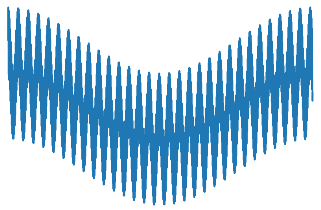
\includegraphics[width=0.55\textwidth]{titlepage_image.png}~\\[2cm]
% Title
\HRule \\[0.4cm]
{ \LARGE 
  \textbf{Project Report for ECE 351}\\[0.4cm]
  \emph{Lab 9: Fast Fourier Transform}\\[0.4cm]
}
\HRule \\[1.5cm]
% Author
{ \large
  Andrew Gibson \\[0.1cm]
 28 March 2023\\[0.1cm]
  \url{https://github.com/gibs0630/ECE351\_Code}\\[0.1cm]
  \url{https://github.com/gibs0630/ECE351\_Reports}\\[0.1cm]
  %#\texttt{user@cut.ac.cy}
}
\vfill
%\textsc{\Large Cyprus University of Technology}\\[0.4cm]\textsc{\large Department of Electrical Engineering,\\Computer Engineering \& Informatics}\\[0.4cm]
% Bottom
{\large }
 
\end{center}
\end{titlepage}
%\begin{abstract}
%\lipsum[1-2]
%\addtocontents{toc}{\protect\thispagestyle{empty}}
%\end{abstract}
\newpage
%===========================================================
\tableofcontents
\addtocontents{toc}{\protect\thispagestyle{empty}}
\newpage
\setcounter{page}{1}
%===========================================================
%===========================================================
\section{Introduction}\label{sec:intro}
With Python, it is possible to apply a filter on a signal that has already been measured and stored.  Being able to do post-processing is important for analysing important details in a signal.

\section{Equations}\label{sec:lit-rev}
Formula's used

Fourier's series
\[x(t) = \sum_{n=-\infty}^\infty \left[ \frac {1}{T} X\left(n \frac{2\pi}{T}\right) e^{j n \frac{2\pi}{T} t}\right]\]


equations from the lab
\[H(s) = \frac{\frac{1}{RC}s}{s^2+\frac{1}{RC}s+\frac{1}{LC}}\]

\[f_1(t) = cos(2\pi*100t) + cos(2\pi*3024t)+sin(2\pi850000t)\]



\section{Methodology}\label{sec:meth}
This lab had us create bode plots of a transfer function and analyze their effect on a signal. W used Python to generate in the $\omega$ domain the frequency response and phase shift of a transfer function. Then we compared it with the outputs from a few libraries available.

\section{Results}\label{sec:res}
\subsection*{Part 1}


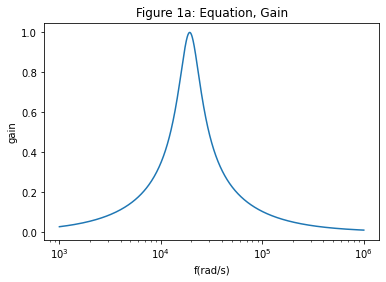
\includegraphics[width=0.8\textwidth]{Figure 1a.png}\\
Figure 1a shows the magnitude of the transfer function for a given frequency using hand calculations. \\

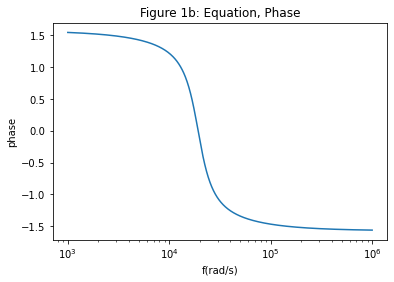
\includegraphics[width=0.8\textwidth]{Figure 1b.png}\\
Figure 1b shows the phase of the transfer function for a given frequency using hand calculations.\\

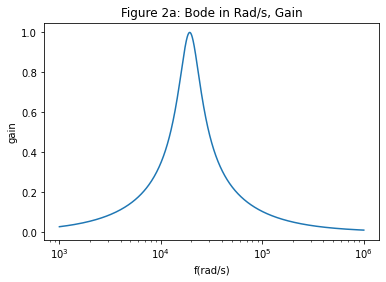
\includegraphics[width=0.8\textwidth]{Figure 2a.png}\\
Figure 2a shows the magnitude of the transfer function for a given frequency using the scipy.signal.bode function.\\

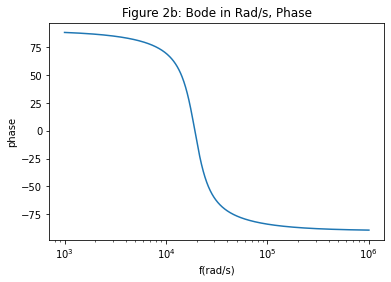
\includegraphics[width=0.8\textwidth]{Figure 2b.png}\\
Figure 1b shows the phase of the transfer function for a given frequency using the scipy.signal.bode function.\\

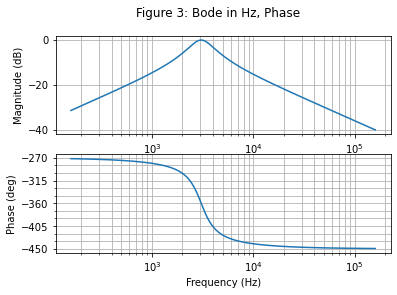
\includegraphics[width=0.8\textwidth]{Figure 3.png}\\
Figure 3 shows the bode plots of the transfer function for a given frequency using the control.TransferFunction function and the control.bode function. The magnitude here is in a scale of dB instead of linear.\\

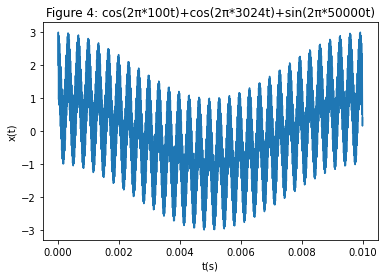
\includegraphics[width=0.8\textwidth]{Figure 4.png}\\
Figure 4 shows the time domain of a signal that will be passed through the transfer function.\\

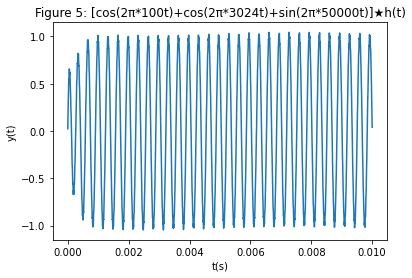
\includegraphics[width=0.8\textwidth]{Figure 5.png}\\
Figure 5 shows the time domain output; notice that the low frequency signal (which causes the largest wave) is not not present, and the high frequency (which causes the sinusoidal to appear solid in color) is also not present. The start ramps up in amplitude because of an artifact from not having data-points before t=0.\\



\section{Questions}\label{sec:res}

\Q Explain how the filter and filtered output in Part 2 makes sense given the Bode plots from Part 1. Discuss how the filter modifies specific frequency bands, in Hz.
\A  The filter makes since when consulting the bode plot. in the original signal, there were three super-positioned sinusoidal with different frequencies. According to the bode plot for magnitude, both the 100Hz and 50000Hz would be attenuated, reducing them to -30 dB relative to the input signal.

\Q Discuss the purpose and workings of scipy.signal.bilinear() and scipy.signal.lfilter()
\A The scipy.signal.biliner function is suppose to convert a signal from the s-domain to the z domain, where the z-domain is composed of discrete timestamps instead of a temporal continuum. The scipy.signal.lfilter function is suppose to do discrete convolution but with a time-domain input and a z-domain filter and then output the filtered output in the time-domain.

\Q What happens if you use a different sampling frequency in scipy.signal.bilinear() than you used for the time-domain signal?
\A If a different sampling frequency is used, then the function may not attenuate certain signals, or it may temporal stretch a signal, or produce artifacts (such as oscillating amplitude for a certain frequency, a wah-wah like effect). For example if the sampling frequency was 3 times that of the input signal sampling frequency then something like this could occur.


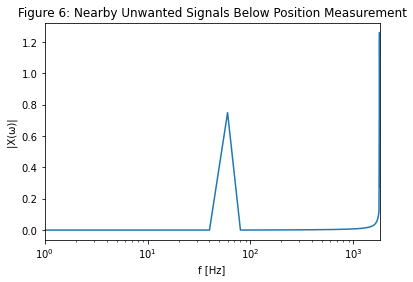
\includegraphics[width=0.8\textwidth]{Figure 6.png}\\
Figure 6 shows that having a miss-match of sampling frequency has undesired effects.

\Q Leave any feedback on the clarity of lab tasks, expectations, and deliverables
\A There was some minor clarity issue with what the variable fs was.



\section{Conclusion}\label{sec:res}
When conducting analysis, it is important to be able to present the findings.  sometimes those finding are hidden behind noise because of a too wide of a viewed domain or because of error caused by the inherit nature of the computers.



%\lipsum[7-8]\cite{knuthwebsite}
%===========================================================
%===========================================================
\bibliographystyle{ieeetr}
\bibliography{refs}
\end{document} 
Annotations











